\documentclass[
	% -- opções da classe memoir --
	12pt,				% tamanho da fonte
	openright,			% capítulos começam em pág ímpar (insere página vazia caso preciso)
	oneside,			% para impressão em frente e verso. Oposto a oneside
	a4paper,			% tamanho do papel.
	% -- opções da classe abntex2 --
	chapter=TITLE,		% títulos de capítulos convertidos em letras maiúsculas
	section=TITLE,		% títulos de seções convertidos em letras maiúsculas
	subsection=TITLE,	% títulos de subseções convertidos em letras maiúsculas
	subsubsection=TITLE,% títulos de subsubseções convertidos em letras maiúsculas
	% -- opções do pacote babel --
	english,			% idioma adicional para hifenização
	brazil				% o último idioma é o principal do documento
	]{abntex2}


% ---
% Pacotes básicos 
% ---
%\usepackage{lmodern}			% Usa a fonte Latin Modern
\usepackage{mathptmx}			% Usa a fonte Times New Roman
%\usepackage{helvet}			% Fonte Parecida com Arial
\usepackage[T1]{fontenc}		% Selecao de codigos de fonte.
\usepackage[utf8]{inputenc}		% Codificacao do documento (conversão automática dos acentos)
\usepackage{lastpage}			% Usado pela Ficha catalográfica
\usepackage{indentfirst}			% Indenta o primeiro parágrafo de cada seção.
\usepackage{color}				% Controle das cores
\usepackage{graphicx}			% Inclusão de gráficos
\usepackage{subcaption}			% Inclusão de gráficos lado a lado
\usepackage{microtype} 			% para melhorias de justificação
\usepackage{tabularx,ragged2e}	% Para inserir tabelas
\usepackage{multirow}			% Para mesclar células
\usepackage[dvipsnames,table,xcdraw]{xcolor}		% Permite adicionar cores nas linhas de tabelas
\usepackage{fancyvrb}			% Permite adicionar arquivos de texto
\usepackage[portuguese, ruled, linesnumbered]{algorithm2e} % Uso de algoritmos
\usepackage{amsfonts}			% Permite usar notação de conjuntos
\usepackage{amsmath}			% Permite citar equações
\usepackage{amsthm}				% Permite criar teoremas e experimentos
\usepackage[font={bf, small}, labelsep=endash, labelfont=bf]{caption}	% Faz legenda de figuras ficarem em negrito
\usepackage{cancel}				% Permite fazer expressão tendendo a zero
\usepackage{epstopdf}			% Converte eps para pdf
\usepackage[final]{pdfpages}
\usepackage{hyphenat}
\usepackage{fancyhdr}
\usepackage{longtable}
\usepackage{graphicx}

\newcolumntype{L}{>{\RaggedRight\arraybackslash}X}
% ---
		
% ---
% Pacotes adicionais, usados apenas no âmbito do Modelo Canônico do abnteX2
% ---
\usepackage{lipsum}				% para geração de dummy text
% ---

% ---
% Pacotes de citações
% ---
%\usepackage[brazilian,hyperpageref]{backref}	 % Paginas com as citações na bibl
\usepackage[alf, abnt-emphasize=bf]{abntex2cite}	% Citações padrão ABNT

% ---
% Customizações para o layout da UFPA
% ---
\usepackage{modelo-ufpa/ufpa}

\tolerance=1
\emergencystretch=\maxdimen
\hyphenpenalty=10000
\hbadness=10000
\hyphenchar\font=-1
\sloppy
\renewcommand{\ABNTEXchapterfontsize}{\normalsize}
\renewcommand{\ABNTEXsectionfontsize}{\normalsize}
\renewcommand{\ABNTEXsubsectionfontsize}{\normalsize}
\renewcommand{\ABNTEXsectionfont}{}
\renewcommand{\ABNTEXsubsectionfont}{}

\renewcommand{\chaptername}{ }
%\renewcommand{\familydefault}{\sfdefault} % usar apenas se usar a fonte helvet

% Muda o título de lista de ilustrações para lista de figuras
\addto\captionsbrazil{%
  \renewcommand{\listfigurename}%
    {Lista de Ilustrações}%
	\renewcommand{\listtablename}%
    {Lista de Tabelas}%
}

\fancypagestyle{ultima}{
\fancyhead{}
\fancyfoot{}
\rhead{\thepage}
}

% Permite utilizar figuras sem precisar colocar o caminho absoluto
\graphicspath{{imagens/}}

% Define o ambiente de experimentos
\theoremstyle{definition}
\newtheorem{experimento}{Experimento}[section]
\newcommand{\experimentoautorefname}{Experimento}

% --- 
% CONFIGURAÇÕES DE PACOTES
% --- 

% ---
% Configurações do pacote backref
% Usado sem a opção hyperpageref de backref
%\renewcommand{\backrefpagesname}{Citado na(s) página(s):~}
% Texto padrão antes do número das páginas
%\renewcommand{\backref}{}
% Define os textos da citação
%\renewcommand*{\backrefalt}[4]{
%	\ifcase #1 %
%		Nenhuma citação no texto.%
%	\or
%		Citado na página #2.%
%	\else
%		Citado #1 vezes nas páginas #2.%
%	\fi}%
% ---

% ---
% Informações de dados para CAPA, FOLHA DE ROSTO e FICHA CATALOGRÁFICA
% ---
\universidade{CENTRO UNIVERSITÁRIO SERRA DOS ÓRGÃOS - UNIFESO}
\instituto{CENTRO DE CIÊNCIA E TECNOLOGIA - CCT}
\curso{CURSO DE BACHARELADO EM CIÊNCIA DA COMPUTAÇÃO}
\titulo{Plataforma web para monitoramento de indicadores de saúde pública}
\autor{Ariel Zimbrão}
\local{TERESÓPOLIS}
\data{2019}
\orientador{Prof. Hermano Lustrosa}
\coorientador{Prof. Leandro Chermicharo} %CASO HAJA UM
\tipotrabalho{Monografia}
\preambulo{Trabalho de Conclusão de Curso apresentado ao Centro Universitário Serra dos Órgãos como requisito obrigatório para obtenção do título de Bacharel em Ciência da Computação.}
\sobrenome{Zimbrão}
\nome{Ariel}% APENAS O PRIMEIRO NOME SEM SOBRENOME
\palavraschave{%
Gestão Pública,
Saúde Pública,
Data Lake.
}

\datadadefesa{Data da Defesa: 28 de Novembro de 2019}% PREENCHER COM O DATA DA DEFESA}
%\conceito{Conceito: Excelente}
\faculdadedoorientador{FACULDADE DO ORIENTADOR} %
\titulacaodoorientador{MSc}%Coloque abreviado a titulação do seu Orientador
\faculdadedocoorientador{FACULDADE DO COORIENTADOR}
\titulacaodocoorientador{DSc}
\primeiromembrodabanca{NOME DO PRIMEIRO MEMBRO DA BANCA}
\titulacaodoprimeiromembro{DSc}
\faculdadedoprimeiromembrodabanca{FACULDADE DO PRIMEIRO MEMBRO DA BANCA}
\segundomembrodabanca{NOME DO SEGUNDO MEMBRO DA BANCA}
\titulacaodosegundomembro{DSc}
\faculdadedosegundomembrodabanca{FACULDADE DO SEGUNDO MEMBRO DA BANCA}
% ---

% ---
% Configurações de aparência do PDF final

% alterando o aspecto da cor azul
\definecolor{blue}{RGB}{41,5,195}

% informações do PDF

\makeatletter
\hypersetup{
     	%pagebackref=true,
		pdftitle={\imprimirtitulo}, 
		pdfauthor={\imprimirautor},
    	pdfsubject={\imprimirpreambulo},
	    pdfcreator={LaTeX with abnTeX2},
		pdfkeywords={\imprimirpalavraschave}, 
		colorlinks=true,       		% false: boxed links; true: colored links
    	linkcolor=black,          	% color of internal links
    	citecolor=black,        		% color of links to bibliography
    	filecolor=magenta,      		% color of file links
		urlcolor=black,
		bookmarksdepth=4,
        breaklinks=true
}
\makeatother


% --- 

% --- 
% Espaçamentos entre linhas e parágrafos 
% --- 

% O tamanho do parágrafo é dado por:
\setlength{\parindent}{1.5cm}

% Controle do espaçamento entre um parágrafo e outro:
\setlength{\parskip}{0.2cm}  % tente também \onelineskip

% ---
% compila o indice
% ---
\makeindex
% ---

% ----
% Início do documento
% ----
\begin{document}

\nocite{Vrs:2018}
% Seleciona o idioma do documento (conforme pacotes do babel)
%\selectlanguage{english}
\selectlanguage{brazil}

% Retira espaço extra obsoleto entre as frases.
\frenchspacing 


% ----------------------------------------------------------
% ELEMENTOS PRÉ-TEXTUAIS
% ----------------------------------------------------------
% \pretextual

% ---
% Capa
% ---
\imprimircapa
% ---

% ---
% Folha de rosto
% ---
\imprimirfolhaderosto
% ---

% ---
% Inserir a ficha bibliografica
% ---
% A biblioteca da universidade lhe fornecerá um PDF
% com a ficha catalográfica definitiva após a defesa do trabalho. Quando estiver
% com o documento, salve-o como PDF no diretório do seu projeto e substitua todo
% o conteúdo de implementação deste arquivo pelo comando abaixo:

%\begin{fichacatalografica}
%    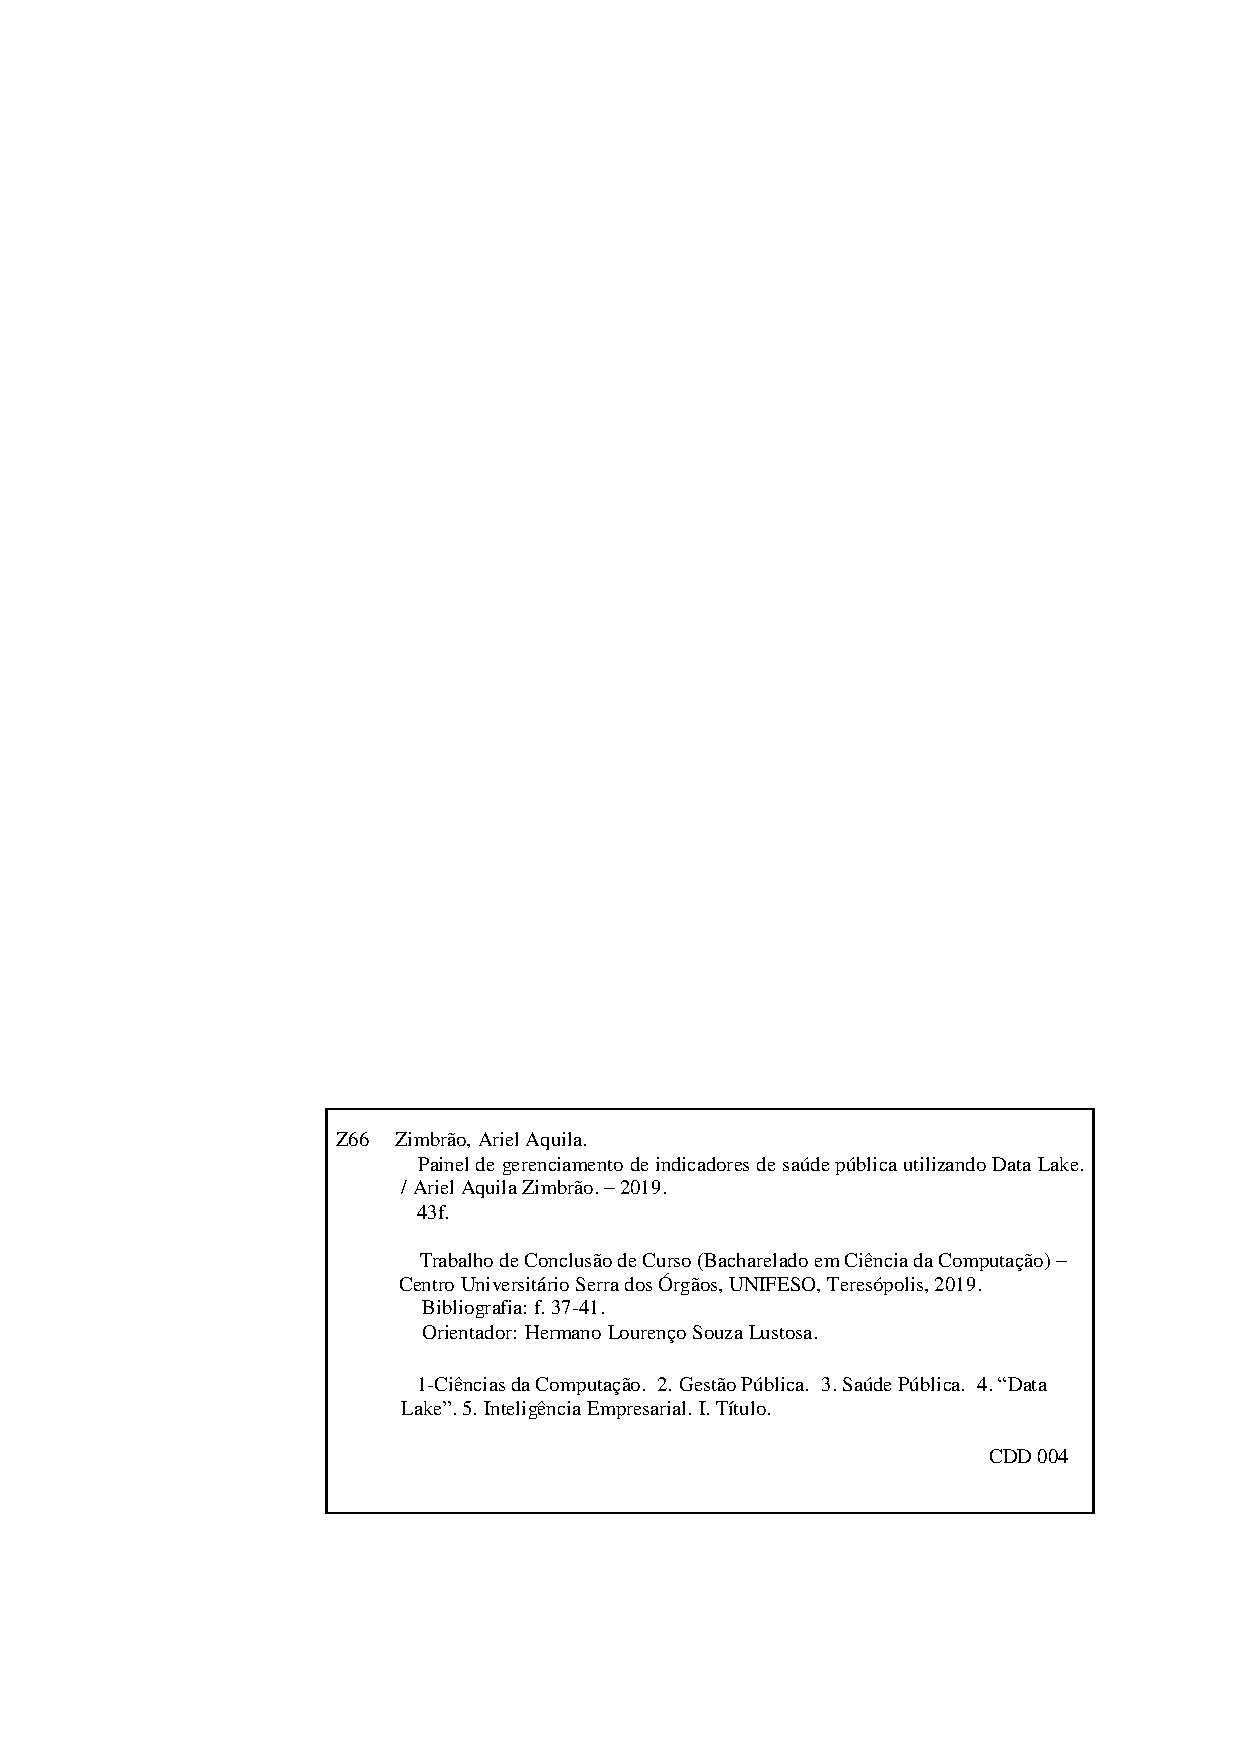
\includepdf{fichacatalografica.pdf}
%\end{fichacatalografica}


\newpage
% ---
% ---

% ---
% Inserir folha de aprovação
% ---
%
\begin{folhadeaprovacao}
\imprimirfolhadeaprovacao
\end{folhadeaprovacao}


% ---

% ---
% Dedicatória
% ---

% ESCREVA A SUA DEDICATORIA A DEDICATORIA QUE SE ENCONTRA NO ARQUIVO E APENAS UM EXEMPLO. ESCOLHA A DEDICATORIA QUE MAIS LHE AGRADAR. LEMBRE-SE DE UTILIZAR AS '\\' PARA PULAR LINHAS

\begin{dedicatoria}
   \vspace*{\fill}
   \flushright
   %\noindent
   \textit{Este trabalho é dedicado às crianças adultas que,\\
   quando pequenas, sonharam em se tornar cientistas. \\
   - Lauro César em abnTeX2}
\end{dedicatoria}
% ---

% ---
% Agradecimentos
% ---
\begin{agradecimentos}

Escreva aqui o seus agradecimentos da maneira que melhor lhe convêm.

\end{agradecimentos}
% ---

% ---
% Epígrafe
% ---

% ESCREVA A SUA EPÍGRAFE A MESMA QUE SE ENCONTRA NO ARQUIVO E APENAS UM EXEMPLO. ESCOLHA A EPÍGRAFE QUE MAIS LHE AGRADAR. LEMBRE-SE DE UTILIZAR AS '\\' PARA PULAR LINHAS

\begin{epigrafe}
    \vspace*{\fill}
	\begin{flushright}
		\textit{``Que todos os nossos esforços estejam sempre focados no desafio à impossibilidade.\\ Todas as grandes conquistas humanas vieram daquilo que parecia impossível.''\\
		(Charles Chaplin)}
	\end{flushright}
\end{epigrafe}
% ---

% ---
% RESUMOS
% ---


% ---

% ---
% inserir lista de ilustrações
% ---
% UTILIZE CASO HAJA FIGURAS NA MONOGRAFIAS. EM QUASO DE AUSENCIA DE FIGURAS COMENTAR COM AS 3 LINHAS DE CODIGOS UTILIZANDO O '%'.
\pdfbookmark[0]{\listfigurename}{lof}
\listoffigures*
\cleardoublepage
% ---

% ---
% inserir lista de quadros
% ---
% UTILIZE CASO HAJA QUADROS NA MONOGRAFIAS. EM QUASO DE AUSENCIA DE QUADROS COMENTAR COM AS 3 LINHAS DE CODIGOS UTILIZANDO O '%'.

\pdfbookmark[0]{\listofquadrosname}{loq}
\listofquadros*
\cleardoublepage
% ---

% ---
% inserir lista de tabelas
% ---

% UTILIZE QUASE HAJA TABELAS NA MONOGRAFIAS. EM QUASO DE AUSENCIA DE TABELAS COMENTAR COM AS 3 LINHAS DE CODIGOS UTILIZANDO O '%'.

\pdfbookmark[0]{\listtablename}{lot}
\listoftables*
\cleardoublepage
% ---

% ---
% inserir lista de algoritmos
% ---

% UTILIZE CASO HAJA ALGORITMOS NA MONOGRAFIAS. EM QUASO DE AUSENCIA DE ALGORITMOS COMENTAR COM AS 3 LINHAS DE CODIGOS UTILIZANDO O '%'.

\pdfbookmark[0]{\listalgorithmcfname}{loa}
\imprimirlistadealgoritmos
\cleardoublepage
% ---

% ---
% inserir lista de abreviaturas e siglas
% ---
% DEVE SER PREENCHIDA A MÃO LEMBRE-SE DE MANTER EM ORDEM ALFABETICA.
\begin{siglas}
  \item[ABNT] Associação Brasileira de Normas Técnicas
\end{siglas}
% ---

% ---
% inserir lista de símbolos
% ---
% DEVE SER PREENCHIDA A MÃO LEMBRE-SE DE MANTER EM ORDEM ALFABETICA.
\begin{simbolos}
  \item[$ \theta $] Letra grega maiúscula theta
\end{simbolos}
% ---

% resumo em português
\setlength{\absparsep}{18pt} % ajusta o espaçamento dos parágrafos do resumo
\begin{resumo}

Escreva aqui o resumo do seu trabalho. Lembre-se escreva o resumo por ultimo na monografia. 

 \textbf{Palavras-chave}: \imprimirpalavraschave
\end{resumo}

% resumo em inglês
\begin{resumo}[Abstract]
 \begin{otherlanguage*}{english}
   Escreva aqui o seu abstract (Resumo em inglês)

   \vspace{\onelineskip}
 
   \noindent 
   \textbf{Keywords}: Keywords1. Keywords2. Keywords3.
 \end{otherlanguage*}
\end{resumo}

% ---
% inserir o sumario
% ---
\pdfbookmark[0]{\contentsname}{toc}
\tableofcontents*
\cleardoublepage
% ---



% ----------------------------------------------------------
% ELEMENTOS TEXTUAIS
% ----------------------------------------------------------
\textual
\pagestyle{simple}

% ----------------------------------------------------------
% Introdução
% ----------------------------------------------------------
\chapter{Introdução}

Escreva aqui sua introdução. para facilitar na escrita aqui vai um dica:

Para pular os parágrafos basta dar um espaço entre os itens que você quer como paragrafo igual foi feito nesse exemplo.

\chapter{FUNDAMENTAÇÃO TEÓRICA}

Escreva aqui sua fundamentação teórica.

\section{SEÇÃO 1}

Deixo aqui uma dica para criar seções, subseções e subsubseções basta utilizar os comandos section, subsection e subsubsection junto de um \ .

\begin{figure}[!h]
\centering
\caption{Escreva aqui o titulo da sua figura}

\includegraphics [scale=0.5]{UNIFESO.png} %coloque suas figuras na pasta imagem e mude o nome do aqui nessa parte. utilize o comando scale para alterar a escala da imagem
\legend{Fonte: \citeauthoronline{unifeso:2018}, \citeyear{unifeso:2018}}
\label{unifeso} % a escreva o nome qualquer a sua figura. Esse nome sera usado para referenciar a figura com o comando \ref{unifeso}
\end{figure}

Utilize o comando \ref{unifeso} para referenciar as suas Figuras.
exemplo: Figura \ref{unifeso}.


\chapter{METODOLOGIA E DESENVOLVIMENTO}

Escreva aqui a metodologia adotada no seu trabalho

% ----------------------------------------------------------
% Considerações Finais
% ----------------------------------------------------------
\chapter{Conclusão}

Escreva a sua conclusão do seu trabalho


% ----------------------------------------------------------
% ELEMENTOS PÓS-TEXTUAIS
% ----------------------------------------------------------
\postextual
% ----------------------------------------------------------

% ----------------------------------------------------------
% Referências bibliográficas
% ----------------------------------------------------------
\bibliography{bibliografia}
% ---


% ----------------------------------------------------------
% Apêndices
% ----------------------------------------------------------

% ---
% Inicia os apêndices
% ---
\begin{apendicesenv}
	
	% Imprime uma página indicando o início dos apêndices
	\partapendices
	
% ----------------------------------------------------------
\chapter{Exemplo}
% ----------------------------------------------------------
	
\end{apendicesenv}
% ---

% ----------------------------------------------------------
% Anexos
% ----------------------------------------------------------

% ---
% Inicia os anexos
% ---
\begin{anexosenv}
	
	% Imprime uma página indicando o início dos anexos
	\partanexos
	
	% ---
    \chapter{Exemplo}
    % ---
	
\end{anexosenv}

\end{document}
